\documentclass[14pt, a4paper, oneside]{extarticle}
\usepackage[utf8]{inputenc}
\usepackage[english, russian]{babel}
\usepackage[T1, T2A]{fontenc}
\usepackage{titlesec}
\usepackage{hyperref}
\usepackage[left=3cm,right=2cm,top=2cm,bottom=2cm,bindingoffset=0cm]{geometry}
\usepackage{indentfirst}
\usepackage{graphicx}
\usepackage{enumitem}
\usepackage{array}
\usepackage[justification=centering]{caption}
\usepackage{float}
\graphicspath{ {./images/} }
\tolerance=10000 % разреженность строки
\linespread{1.4} % интерлиньяж
\hypersetup{
    colorlinks=true,
    linkcolor=black,
    urlcolor=black,
    citecolor=black,
}

\title{Masters Term Paper}
\author{Evgenia Abdullaeva}
\date{May 2022}

\begin{document}
\begin{titlepage}
    \centering
        \begin{figure}[H]
            \centering
            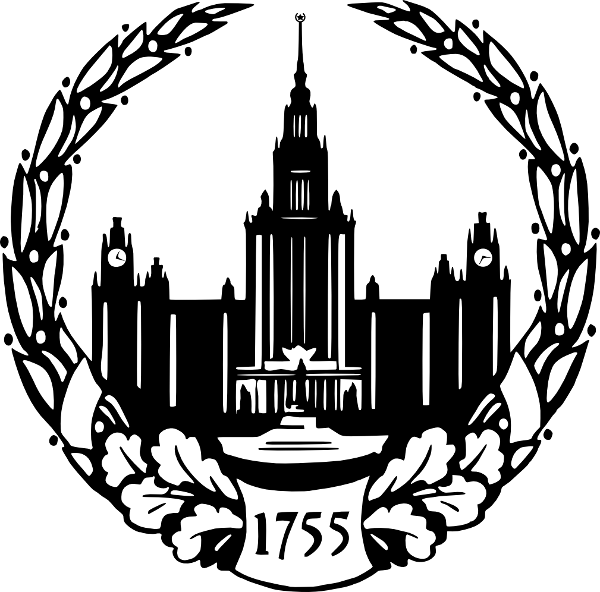
\includegraphics[scale=1.6]{msu-logo}
        \end{figure}
        Московский государственный университет имени М.В. Ломоносова\\
        \vspace{0.5cm}
        Факультет космических исследований\\
        Магистерская программа <<Методы и технологии дистанционного зондирования Земли>>\\
        \vfill
        \textbf{КУРСОВАЯ РАБОТА\\
        на тему: <<Развитие методов классификации и оценки значимости признаков на основе случайных лесов в контексте задачи картографирования земного покрова России>>}\\
        \vfill
        Абдуллаева Евгения Гасановна\\
        \vspace{0.5cm}
        Научный руководитель:\\
        к.т.н. Хвостиков Сергей Антонович
        \vfill
        Москва, 2022 г.
\end{titlepage}

\begin{abstract}
Аннотация на английском + презентация для английского
\end{abstract}
\selectlanguage{english}
\begin{abstract}

\end{abstract}
\selectlanguage{russian}
\setcounter{page}{2}
\newpage

\tableofcontents
\newpage

\section{Введение}
% Постановка проблемы, цель работы
СМЫСЛ \\
Зачем классифицировать земной покров? \\
Зачем новые методы автоматизации классификации земного покрова? \\
Об алгоритме LAGMA \\
Что-то о машинном обучении в применении к колоссальным объемам спутниковых данных \\

% Актуальность
Ранее к этому набору данных случайные леса не применялись всерьез. Соответственно развитие заключается в применении нового метода классификации, оценке влияния разных параметров/подходов на точность классификации, а также в анализе входных данных, их значимости.

\newpage

\section{Анализ данных}
Инструменты -- источник данных +,

количество элементов, признаки, значения +,

классы, количество элементов классов, легенда классов, диаграмма +, КАК ПОЛУЧЕНЫ КЛАССЫ в выборке (алгоритм LAGMA?)

визуализация классов графиками (box plots) и/или линейный график один на все классы по медианам для каждого признака, отдельные карты для каждого класса, сравнение с реальной картой, объединить одинаковые классы, полная карта всей выборки с легендой

ПРОЧЕСТЬ ДОКУМЕНТАЦИЮ vaex

технические штуки: vaex, набор данных больше размера ОЗУ,

предобработка -- прув, что она не влияет на качество классификации,

\subsection{Источник данных}
В данной работе классификация осуществляется на основе спутниковых данных (стандартного продукта MOD09) 2010 года (весенних, летних и осенних) и 2011 года (зимних), полученных спектрорадиометром Moderate Resolution Imaging Spectroradiometer (MODIS), установленным на спутниках Terra и Aqua. Продукт MOD09 представляет собой данные о спектрально-отражательных характеристиках земной поверхности, геопривязанные и скорректированные на атмосферу. Данные предварительно обработаны для исключения влияния облаков и теней от них путем осреднения значений яркости за сезон, по ним созданы сезонные композиты.

Прибор MODIS разработан для изучения биологических и физических процессов в глобальном масштабе с периодичностью наблюдений в 1-2 дня, в частности, для исследований растительного покрова. MODIS имеет 36 спектральных каналов в диапазоне $\lambda$ = 0,46-14,39 мкм, в том числе информативные для изучения растительности красный ($\lambda$ = 0,62-0,67 мкм) и ближний инфракрасный ($\lambda$ = 0,84-0,88 мкм) каналы с пространственным разрешением 250 м, и ряд каналов с разрешением 500 м, используемых для анализа характеристик растительности и фильтрации облачности. Полоса охвата прибора составляет 2330 км, а покрытие данными измерений всей территории России обеспечивается с периодичностью не реже одного раза в сутки. Таким образом, данные прибора образуют непрерывный однородный архив ежедневных наблюдений в течение более 15 лет, анализ которых может быть эффективно использован для изучения и мониторинга растительного покрова. Данные MODIS успешно используются для создания глобальной карты типов земного покрова \cite{land-cover-mapping-monograph}.

\subsection{Общие сведения о данных}
Данные для классификации представлены в табличном виде. Полный набор данных содержит 74029669 элементов (строк таблицы). Каждый элемент описан 14-ю признаками (столбцы таблицы), содержащими неотрицательные целочисленные значения:

CLASS (значения от 1 до 23) --- индекс класса элемента выборки;

X (значения от 5820 до 40161), Y (значения от 1429 до 20580) --- координаты элемента выборки (индекс пикселя в растровом изображении, размер пикселя --- 230 метров);

WINTER1 (значения от 0 до 10583), WINTER2 (значения от 0 до 10584) --- яркость композитного изображения за зимний сезон в красном канале (RED, $\lambda$ = 0,62-0,67 мкм) и ближнем инфракрасном канале (NIR, $\lambda$ = 0,84-0,88 мкм), соответственно;

SPRING1 (значения от 1 до 8653) --- яркость композитного изображения за весенний сезон в канале RED;

SPRING2 (значения от 1 до 7018) --- яркость композитного изображения за весенний сезон в канале NIR;

SPRING3 (значения от 1 до 5211) --- яркость композитного изображения за весенний сезон в коротковолновом инфракрасном канале (SWIR, $\lambda$ = 1,63-1,65 мкм);

SUMMER1 (значения от 1 до 8653), SUMMER2 (значения от 1 до 6907), SUMMER3 (значения от 1 до 4923) --- яркость композитного изображения за летний сезон в каналах RED, NIR, SWIR, соответственно;

FALL1 (значения от 1 до 8653), FALL2 (значения от 1 до 6907), FALL3 (значения от 1 до 5280) --- яркость композитного изображения за осенний сезон в каналах RED, NIR, SWIR, соответственно.

\subsection{Классифицируемые типы земного покрова}
\subsubsection{Типы земного покрова и их представленность в выборке}
Представленные в наборе данных типы земного покрова включают в себя 19 тематических классов, образующих 5 различных групп земного покрова, а именно:

\begin{enumerate}
    \item Леса:
    \begin{itemize}
        \item[-] Темнохвойные вечнозеленые насаждения (\textit{темнохвойный лес}), в пологе которых не менее 80\% площади крон составляют теневыносливые виды хвойных деревьев, включая ель, пихту и сибирскую сосну (кедр).
        \item[-] Светлохвойные вечнозеленые насаждения (\textit{светлохвойный лес}), в пологе которых не менее 80\% площади крон составляют деревья сосны обыкновенной.
        \item[-] Лиственные насаждения (\textit{лиственный лес}), в пологе которых не менее 80\% площади занимают кроны березы и осины, а также широколиственных пород, включая дуб, липу, ясень, клен, вяз и некоторые другие виды.
        \item[-] Смешанные насаждения с преобладанием хвойных пород (\textit{смешанный лес с преобладанием хвойных}), в которых кроны хвойных деревьев занимают от 60\% до 80\%, а лиственных --- от 20\% до 40\% площади полога.
        \item[-] Смешанные насаждения (\textit{смешанный лес}), в которых площади крон хвойных и лиственных пород деревьев представлены примерно в равных пропорциях (40-60\%) в пологе.
        \item[-] Смешанные насаждения с преобладанием лиственных пород (\textit{смешанный лес с преобладанием лиственных}), в которых кроны лиственных пород деревьев занимают от 60\% до 80\%, а хвойных --- от 20\% до 40\% площади полога.
        \item[-] Хвойные листопадные (лиственничные) насаждения (\textit{хвойный листопадный лес}), в пологе которых кроны деревьев лиственницы занимают более 80\% площади.
        \item[-] \textit{Редины хвойные листопадные} (лиственничные), представляющие собой участки, занятые отдельно стоящими деревьями или разреженными насаждениями лиственницы с проектным покрытием крон менее 20\%.
    \end{itemize}
    \item Травяно-кустарниковая растительность:
    \begin{itemize}
        \item[-] \textit{Луга} --- травяная растительность с продолжительностью вегетационного сезона более 5 месяцев, видовой состав которой характеризуется господством многолетних трав, главным образом злаков и осоковых, в условиях достаточного увлажнения. Площадь проекции крон деревьев и кустарников на земную поверхность составляет менее 20\%.
        \item[-] \textit{Степь} --- травяной покров образован преимущественно засухоустойчивыми 
        многолетними дерновинными злаками (ковыль, типчак, полынь, житняк и др.).Встречается большое разнообразие видов степных кустарников и полукустарников, а также короткоцветущих эфемероидов и эфемеров.
        \item[-] Хвойные вечнозеленые кустарники (\textit{хвойный кустарник}) --- кустарниковые заросли или низкоствольные леса из кедрового стланика.
        \item[-] Лиственные кустарники (\textit{лиственный кустарник}) --- сообщество низкорослых и стелющихся кустарников (кустарниковых или карликовых берез, полярных ив и др.).
    \end{itemize}
    \item Тундра:
    \begin{itemize}
        \item[-] \textit{Кустарничковая тундра} --- сухая тундра с редкой фрагментарной растительностью, среди которой доминируют виды альпоарктических кустарничковых сообществ высотой менее 15 см. Распространены также мохово-лишайниковый покров и разнотравье.
        \item[-] \textit{Травянистая тундра} представлена главным образом различными видами трав и мхов, произрастающими на сырых почвах и образующими сплошной растительный покров. Часто встречаются кустарнички высотой до 40 см.
        \item[-] \textit{Кустарниковая тундра} с доминированием кустарников (карликовая береза и различные виды ивы) высотой более 40 см, иногда с примесью можжевельника, ольхи или кедрового стланика.
    \end{itemize}
    \item Водно-болотные комплексы:
    \begin{itemize}
        \item[-] \textit{Болота} --- территории, характеризующиеся избыточным увлажнением с преобладанием растительного покрова из мхов, лишайников, тростника, осоки и некоторых других видов. Часто встречаются участки с наличием редкого (<20\%) древесного полога.
        \item[-] \textit{Прибрежная растительность} --- гидрофильная травяная и древеснокустарниковая растительность по берегам водоемов, часто периодически затопляемая.
    \end{itemize}
    \item Не покрытые растительностью земли:
    \begin{itemize}
        \item[-] \textit{Открытые грунты и выходы горных пород} --- земли, суммарное проективное покрытые которых растительностью всех видов не превышает 20\%.
        \item[-] \textit{Водные объекты} --- речные и озерные внутренние водоемы, а также прибрежные участки открытой воды.
    \end{itemize}
\end{enumerate}

\begin{table}[H]
    \centering
    \caption{Количество представителей тематических классов\\земного покрова в выборке}
    \begin{tabular}{ m{12.1cm}r }
        \textbf{Класс} & \textbf{Количество} \\
        \hline
        Темнохвойный лес & 6153034 \\
        Светлохвойный лес & 4500884 \\
        Лиственный лес & 8734036 \\
        Смешанный лес с преобладанием хвойных & 1025492 \\
        Смешанный лес & 378946 \\
        Смешанный лес с преобладанием лиственных & 1505855 \\
        Хвойный листопадный лес & 22271771 \\
        Редины хвойные листопадные & 3586296 \\
        Луга & 5858059 \\
        Степь & 2091630 \\
        Хвойный кустарник & 1096112 \\
        Лиственный кустарник & 267236 \\
        Кустарничковая тундра & 1943579 \\
        Травянистая тундра & 4893560 \\
        Кустарниковая тундра & 1178381 \\
        Болота & 4657062 \\
        Прибрежная растительность & 9661 \\
        Открытые грунты и выходы горных пород & 2691471 \\
        Водные объекты & 1186604 \\
        \hline
        Всего элементов & 74029669 \\
    \end{tabular}
\end{table}

\begin{figure}[H]
    \caption{Относительное количество представителей тематических классов земного покрова в выборке}
    \centering
    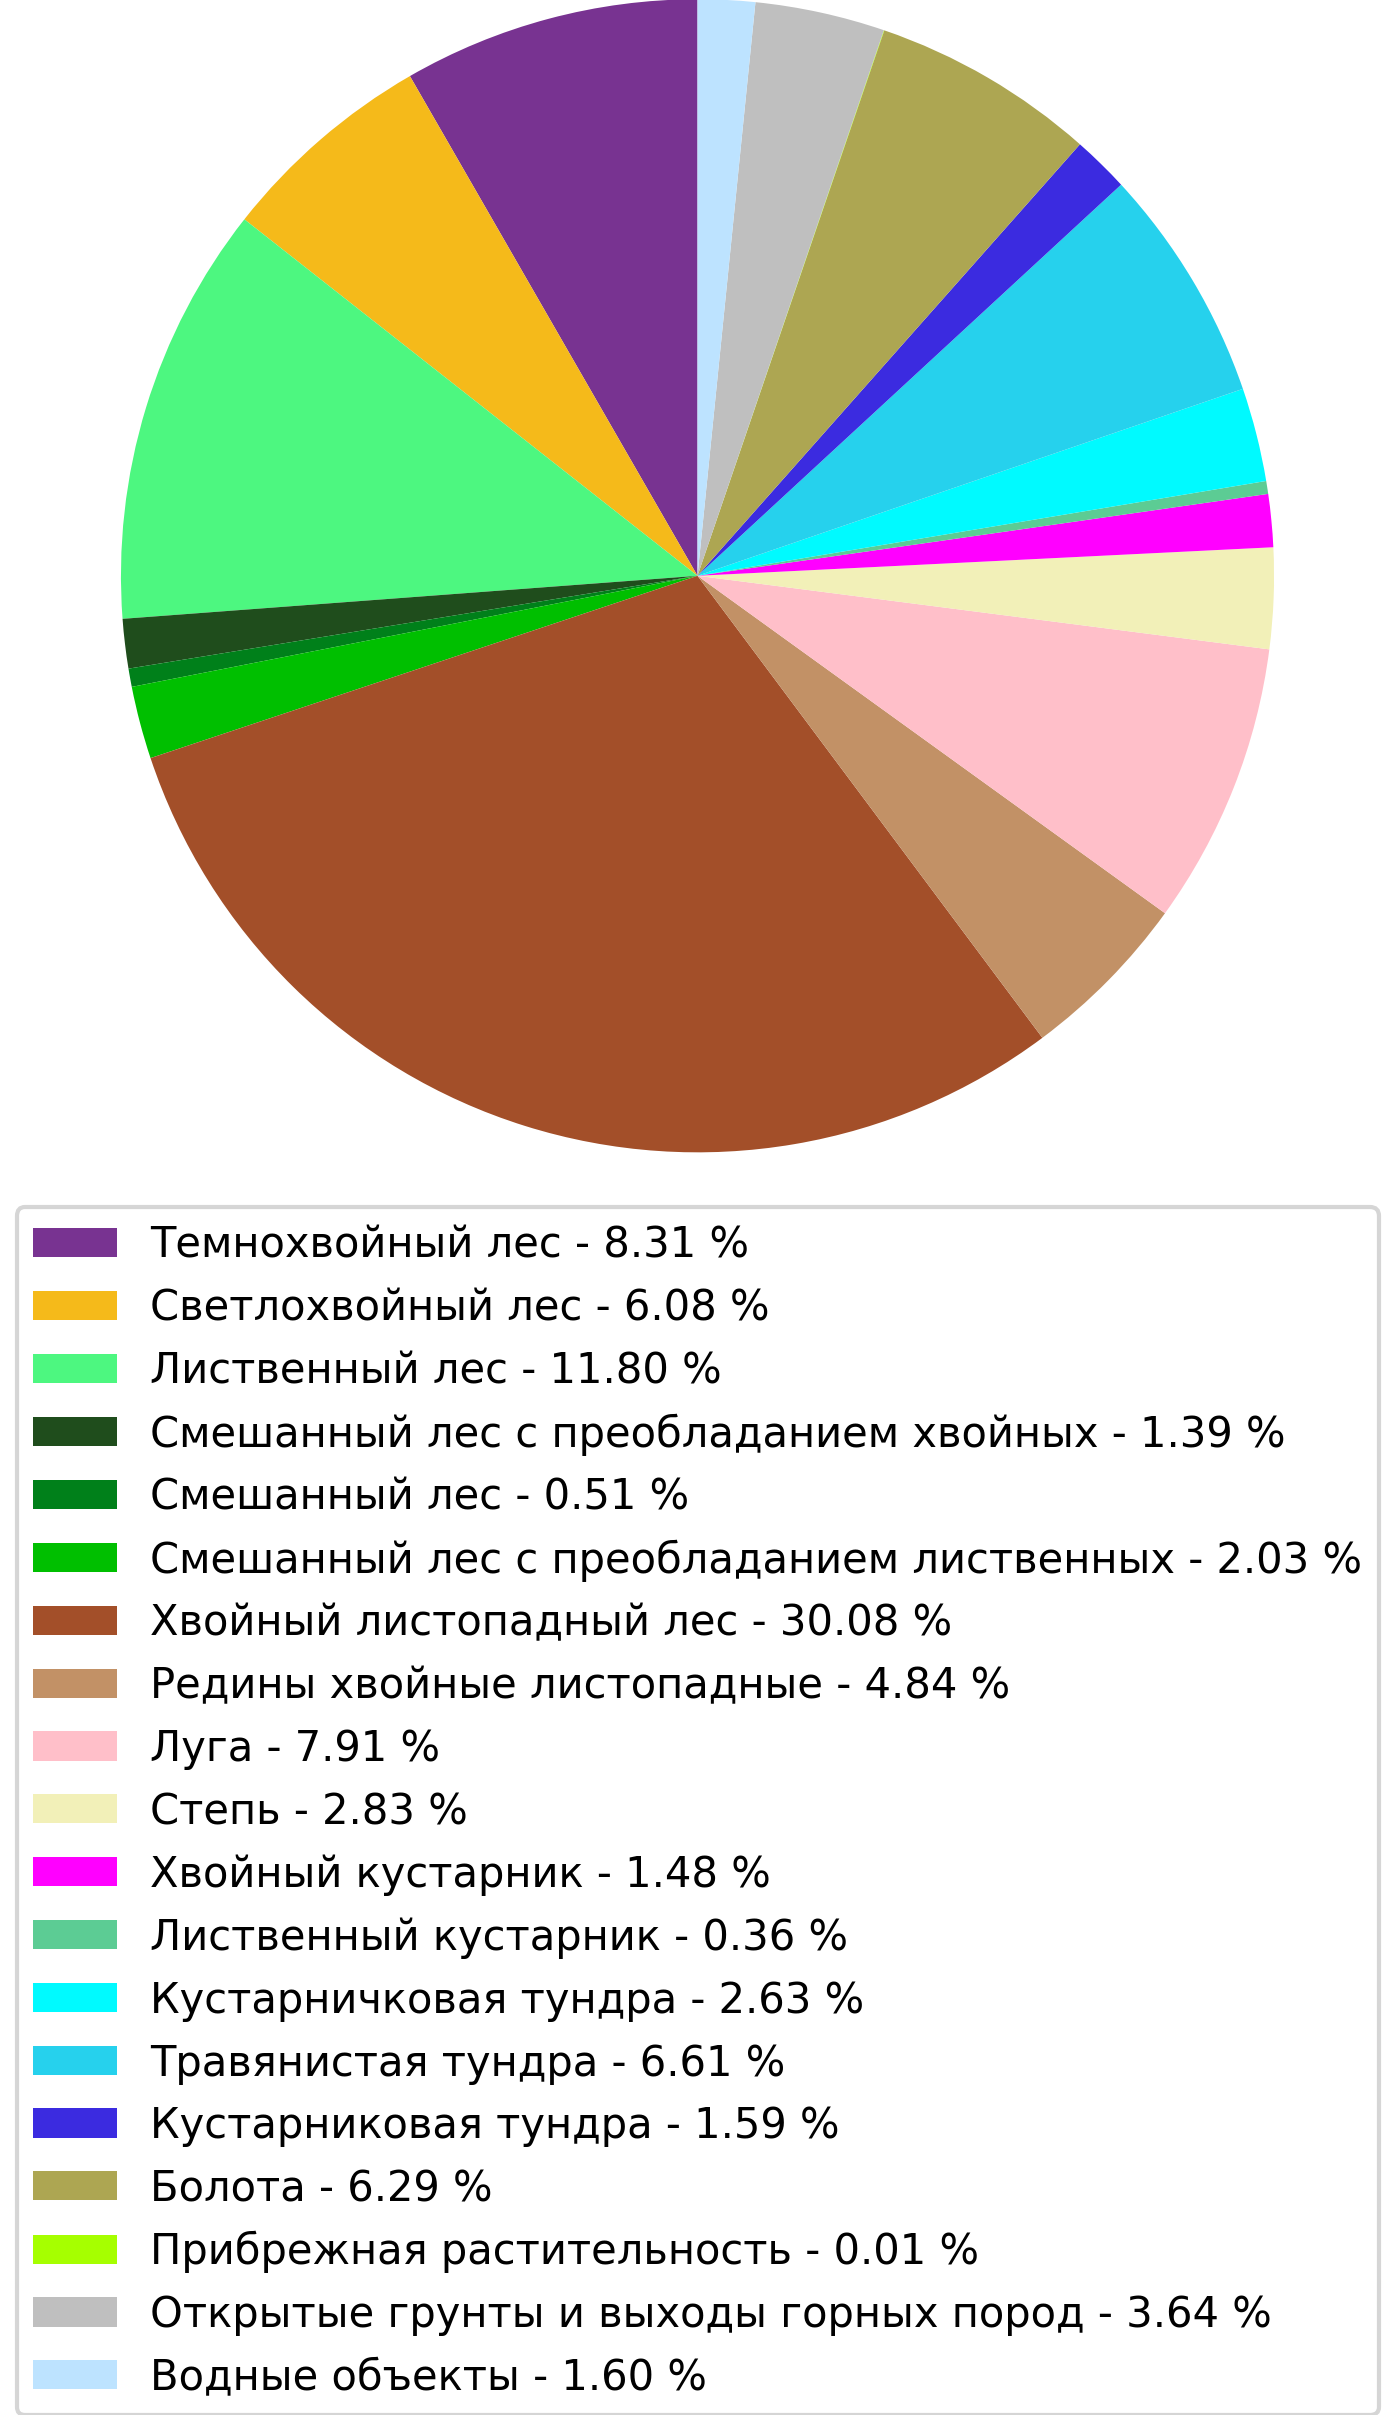
\includegraphics[scale=0.9]{classes-ratio}
\end{figure}

\subsubsection{Визуализация типов земного покрова}
ololo

\subsection{}
\newpage

\section{Классификация земного покрова с помощью модели случайного леса}
МАТЕМАТИЧЕСКАЯ МОДЕЛЬ задачи классификации, определение машинного обучения (с учителем)

Почему случайный лес?

Обучение, проверка на полном наборе данных (нет ли переобучения)

МЕТРИКИ ДЛЯ КЛАССИФИКАЦИИ, визуализировать ошибки на карте, CONFUSION MATRIX

ПОДБОР ОПТИМАЛЬНЫХ ГИПЕРПАРАМЕТРОВ

\newpage

\section{Значимость признаков}
ЗНАЧИМОСТЬ ПРИЗНАКОВ

Методы оценки значимости признаков

Уменьшать количество признаков --- оценивать влияние на качество классификации и время обучения
\newpage

\section{Применение модели случайного леса к полному набору данных}
Применение результатов исследования к полному набору данных, confusion matrix
\newpage

\section{Применение модели случайного леса к карте земного покрова}
Получить табличные данные из изображений (GDAL)

Применить модель к полученным данным, применима ли модель?
\newpage

\section{Заключение}
\newpage

\section{Литература}
\begingroup
\renewcommand{\section}[2]{}
\begin{thebibliography}{20}
    \bibitem{land-cover-mapping-monograph}
    \textit{Барталев С.А., Егоров В.А., Жарко В.О., Лупян Е.А., Плотников Д.Е., Хвостиков С.А., Шабанов Н.В.} Спутниковое картографирование растительного покрова России // ИКИ РАН. 2016. C. 93-110.

    \bibitem{land-cover-mapping-article}
    \textit{Барталев С.А., Егоров В.А., Жарко В.О., Лупян Е.А., Плотников Д.Е., Хвостиков С.А.} Состояние и перспективы развития методов спутникового картографирования растительного покрова России // Современные проблемы дистанционного зондирования Земли из космоса. 2015. Т. 12. № 5. С. 203-221.

    \bibitem{random-forest-in-remote-sensing}
    \textit{Belgiu M., Drăguţ L.} Random forest in remote sensing: A review of applications and future
    directions // ISPRS Journal of Photogrammetry and Remote Sensing. 2016. No. 114. pp. 24-31.
    
    \bibitem{python}
    Документация языка Python\\
    \url{https://docs.python.org/3}
\end{thebibliography}
\endgroup
\newpage

\linespread{1.2}
\section{Приложения}
\newpage

\end{document}
